
%(BEGIN_QUESTION)
% Copyright 2007, Tony R. Kuphaldt, released under the Creative Commons Attribution License (v 1.0)
% This means you may do almost anything with this work of mine, so long as you give me proper credit

An {\it intrinsic safety barrier} circuit is essential for making loop-powered 4-20 mA instrument systems ``intrinsically safe.''  Explain what intrinsic safety means for an instrument system such as this, and also how the components inside the barrier circuit make the circuit intrinsically safe:

$$\includegraphics[width=15.5cm]{i02471x01.eps}$$

Supposing the resistor inside this intrinsic safety barrier has a probability of $2.4 \times 10^{-6}$ of failing open, and the diode has a probability of $1.3 \times 10^{-4}$ of failing shorted, calculate the probability that either of these two failures will interrupt the transmitter's signal from getting to the controller.

\vskip 10pt

Supposing the fuse inside the barrier has a probability of $5.8 \times 10^{-4}$ of failing open.  How does this affect the probability of signal interruption for any barrier component failure?

\vskip 20pt \vbox{\hrule \hbox{\strut \vrule{} {\bf Suggestions for Socratic discussion} \vrule} \hrule}

\begin{itemize}
\item{} A good reasoning technique to apply if you are having difficulty explaining the purpose of something is to explain the converse: what things would be like it that something were {\it not} present.  In this case, explain why the circuit could be unsafe without the barrier in place, assuming certain circuit faults such as opens and shorts in the classified field location.
\item{} Will the presence of an intrinsic safety barrier guarantee safe operation for {\it any} device installed in a classified area, or must the field devices themselves also be designed and rated for intrinsic safety?
\item{} Would the loop-powered transmitter circuit still be considered intrinsically safe if the barrier were not present?  Would it be considered non-incendive?
\item{} Which of the two components inside the barrier poses the greatest risk to reliability, based on the failure probabilities?
\end{itemize}

\underbar{file i02471}
%(END_QUESTION)





%(BEGIN_ANSWER)

The intrinsic safety barrier protects against potential ignition resulting from short-circuits in the field wiring, and from over-voltage from the process controller power supply.  I'll let you explain {\it how} the barrier circuit's components do this!

\vskip 10pt

The probability of either the resistor or the diode interrupting the signal is a logical ``OR'' function, and so the calculation of probability takes this form:

$$\includegraphics[width=15.5cm]{i02471x03.eps}$$

$$P(\hbox{A {\it or} B}) = P(B) + P(A) - P(A) \times P(B)$$

$$P_{interruption} = (2.4 \times 10^{-6}) + (1.3 \times 10^{-4}) - [(2.4 \times 10^{-6})(1.3 \times 10^{-4})] $$

$$P_{interruption} = 1.324 \times 10^{-4}$$

\vskip 10pt

Adding the fuse's fault probability into the mix is another ``OR'' function:

$$\includegraphics[width=15.5cm]{i02471x04.eps}$$

$$P_{interruption} = (1.324 \times 10^{-4}) + (5.8 \times 10^{-4}) - [(1.324 \times 10^{-4})(5.8 \times 10^{-4})] $$

$$P_{interruption} = 7.123 \times 10^{-4}$$


%(END_ANSWER)





%(BEGIN_NOTES)




\vskip 20pt \vbox{\hrule \hbox{\strut \vrule{} {\bf Virtual Troubleshooting} \vrule} \hrule}

This question is a good candidate for a ``Virtual Troubleshooting'' exercise.  Presenting the diagram to students, you first imagine in your own mind a particular fault in the system.  Then, you present one or more symptoms of that fault (something noticeable by an operator or other user of the system).  Students then propose various diagnostic tests to perform on this system to identify the nature and location of the fault, as though they were technicians trying to troubleshoot the problem.  Your job is to tell them what the result(s) would be for each of the proposed diagnostic tests, documenting those results where all the students can see.

During and after the exercise, it is good to ask students follow-up questions such as:

\begin{itemize}
\item{} What does the result of the last diagnostic test tell you about the fault?
\item{} Suppose the results of the last diagnostic test were different.  What then would that result tell you about the fault?
\item{} Is the last diagnostic test the best one we could do?
\item{} What would be the ideal order of tests, to diagnose the problem in as few steps as possible?
\end{itemize}

%INDEX% Safety, intrinsic: passive zener barrier circuit

%(END_NOTES)


